\section{TwoOpt Class Reference}
\label{class_two_opt}\index{TwoOpt@{TwoOpt}}
Inheritance diagram for TwoOpt::\begin{figure}[H]
\begin{center}
\leavevmode
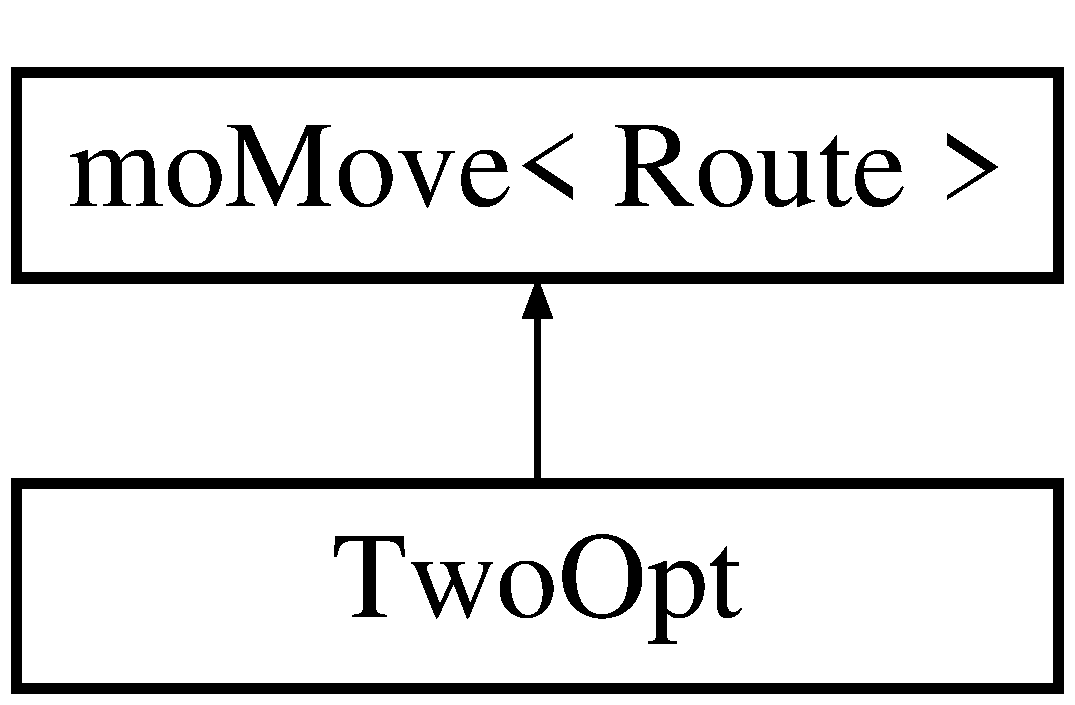
\includegraphics[height=2cm]{class_two_opt}
\end{center}
\end{figure}
\subsection*{Public Member Functions}
\begin{CompactItemize}
\item 
{\bf TwoOpt} {\bf operator!} () const\label{class_two_opt_bc412d9f7fe3617cafef364f860d8d41}

\item 
void {\bf operator()} (Route \&\_\-\_\-route)\label{class_two_opt_ff87d1649a33d42a6d64e8d314ed1af0}

\item 
void {\bf readFrom} (std::istream \&\_\-\_\-is)\label{class_two_opt_feccfecca2a6bd2d3a12afdf3f724be0}

\item 
void {\bf printOn} (std::ostream \&\_\-\_\-os) const\label{class_two_opt_77ea59d81dd829ee3190219fa8659adc}

\end{CompactItemize}


\subsection{Detailed Description}




Definition at line 22 of file two\_\-opt.h.

The documentation for this class was generated from the following files:\begin{CompactItemize}
\item 
two\_\-opt.h\item 
two\_\-opt.cpp\end{CompactItemize}
